
\section{S\"avje et al. (2017)}

% -------------------------------------------------------------------------

\begin{frame}
  \frametitle{S\"avje et al (2017)}
  
  \begin{itemize}
  \item \textbf{Hypothesis:} social norms influence citizens'
    propensity to vote \citep*{gerber2008social}.
  \item \textbf{Goal:} study effectiveness of a postcard intervention
    in increasing voter turnout.  There are six total treatment conditions. 
  \item Introduce \emph{generalized full matching}, which extends full
    matching to the case of categorical treatment with $k$ levels.
  \end{itemize}
  
  \medskip

  Gerber et al. prescreened voters to be included in the study, so the
  original results were not generalizeable to the entire population.
    
\end{frame}

% -------------------------------------------------------------------------

\begin{frame}
  \frametitle{Full matching}
  
  This paper generalizes full
  matching\footnote{\cite{rosenbaum2001,hansen2004,stuart2008}}: \medskip
  
  \begin{itemize}
  \item Construct groups of units that are as homogeneous as possible \medskip 
  \item Require that each group has at least one unit of each
    treatment condition \medskip
  \item So far, only developed for case of binary treatment
  \end{itemize}


  \bigskip

  \emph{All units} are matched to a subclass, hence the term ``full''

\end{frame}

% -------------------------------------------------------------------------

\begin{frame}
  \frametitle{Notation}
  
  \begin{itemize}
  \item Denote the sample of $n$ units by $\U = \{1,2,\ldots,n\}$    \medskip 
  \item Unit $i$ is assigned to treatment condition
    $W_i \in \{1,2,\ldots,k\}$ \medskip 
  \item The vectors $\w_x = \{i : W_i = x\}$ denote sets of units
    assigned to a given treatment condition \medskip 
  \item Matched groups are denoted by $\m$, and the union of matched
    groups is $\M = \{\w_1, \w_2, \ldots \}$ \medskip 
  \item Define an objective function
    $L: \mathcal{M} \rightarrow \mathbb{R}$, where $\mathcal{M}$ is
    the set of possible matches
  \end{itemize}


\end{frame}

% -------------------------------------------------------------------------

\begin{frame}
  \frametitle{Match group constraints}

  Constrain the set of admissible matches $\mathcal{M}$ as follows:

  \medskip 

  \begin{itemize}
  \item Each match group $\m$ must contain $c_x$ no. of units with
    treatment condition $x$ \medskip 
  \item Each match group must contain at least $t \geq \sum_{x=1}^{k}
    c_x$ no. of units overall \medskip 
  \item Union of match groups must contain all units, $\M = \bigcup \m = \U$
  \end{itemize}
  
\end{frame}

% -------------------------------------------------------------------------

\begin{frame}
  \frametitle{Algorithm}
  
  \ldots
  
\end{frame}


% -------------------------------------------------------------------------

\begin{frame}
  \frametitle{Graphical example}
  
  \begin{figure}[ht]
    \centering
    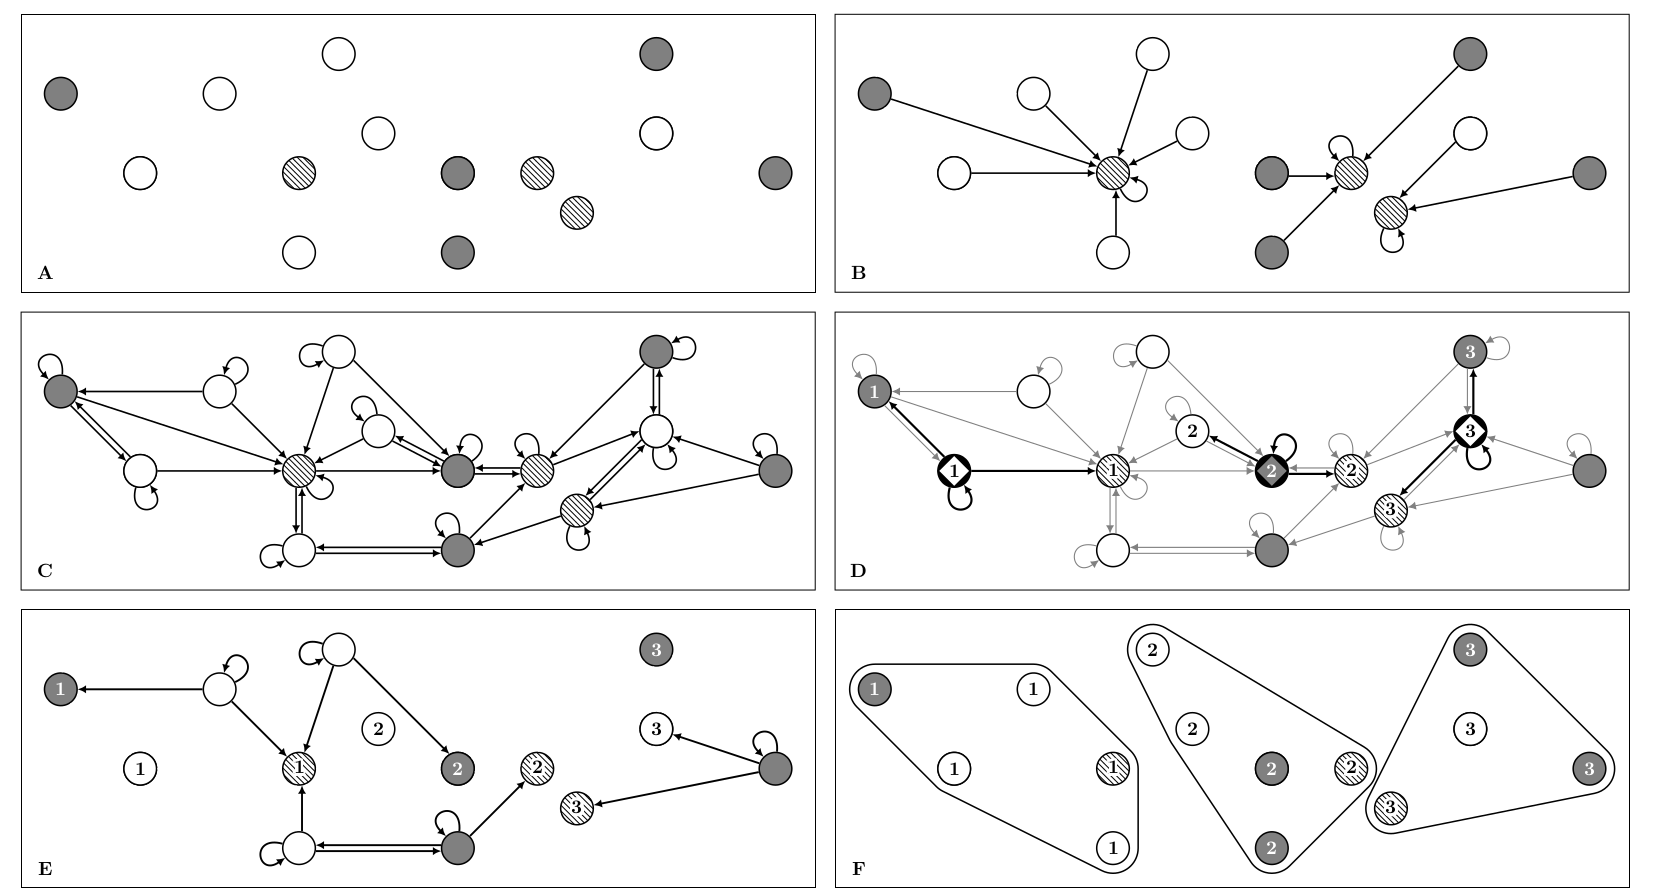
\includegraphics[width=\textwidth]{figures/saevje-network.png}
    % \caption{\label{fig:label} }
  \end{figure}

  
\end{frame}

% -------------------------------------------------------------------------

\begin{frame}
  \frametitle{Properties}

  Let $\M_{\text{alg}}$ be the set of matches resulting from the algorithm

  \begin{block}{Theorem: S\"avje et al. (2019)}
    $$L(\M_\text{alg}) \leq \min_{\M \in \mathcal{M}} 4 L(\M)$$
  \end{block}
  
\end{frame}

% -------------------------------------------------------------------------

\begin{frame}
  \frametitle{Covariate balance}
  
  \begin{figure}[ht]    
    \centering
    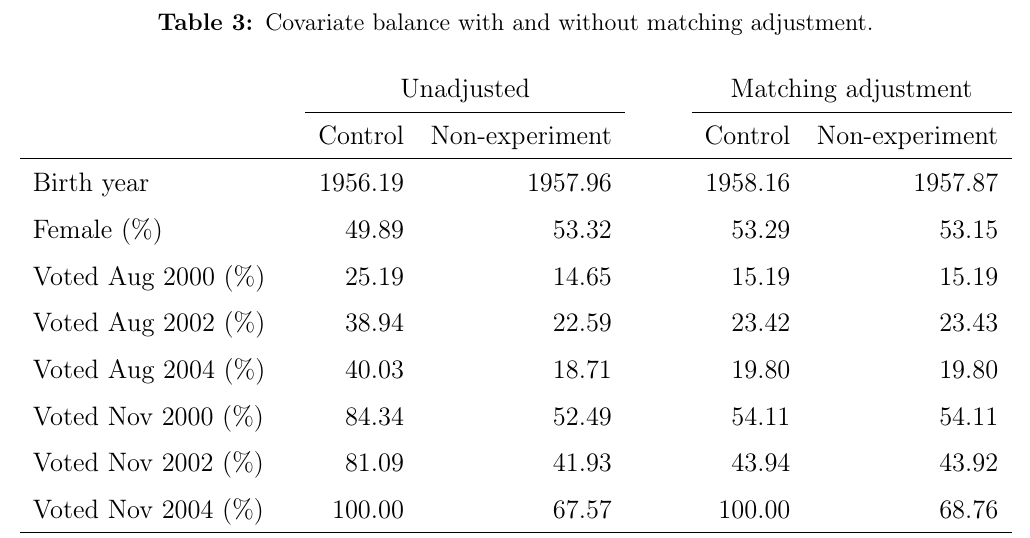
\includegraphics[width=0.99\textwidth]{figures/saevje-table3.png}
    % \caption{\label{fig:label} }
  \end{figure}

  Construct matched groups based on Mahalonobis distance
  
\end{frame}

% -------------------------------------------------------------------------



\begin{frame}
  \frametitle{Results on voter turnout data (1)}
  
  \begin{figure}[ht]    
    \centering
    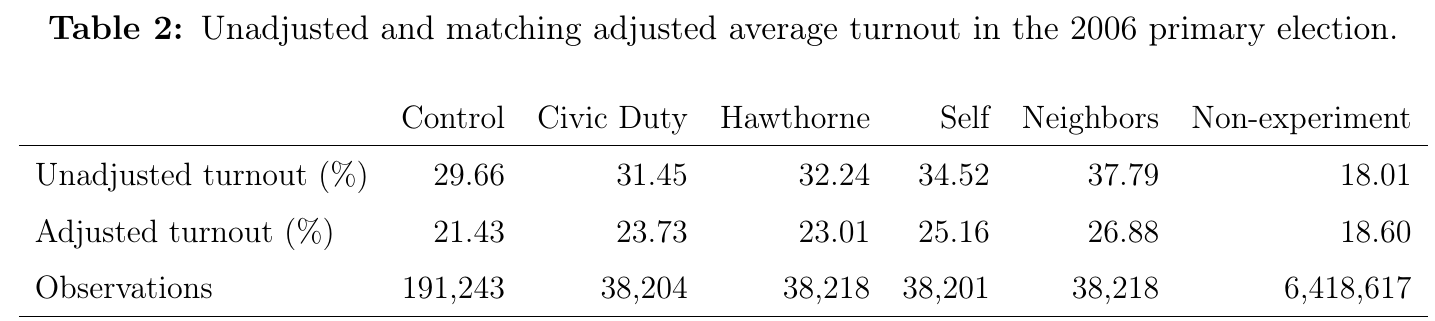
\includegraphics[width=0.99\textwidth]{figures/saevje-table2.png}
    % \caption{\label{fig:label} }
  \end{figure}

  \footnotesize{\emph{The figures [in the second row] should be
      interpreted as estimates of turnout of the six conditions if
      scaled up to the whole population}}

  \normalsize

  \medskip 

  Control and non-experiment groups should be more similar....
  
\end{frame}

% -------------------------------------------------------------------------

\begin{frame}
  \frametitle{Results on voter turnout data (2)}

  Now restrict to units that voted in 2004 election\ldots

  \medskip 

  \begin{figure}[ht]    
    \centering
    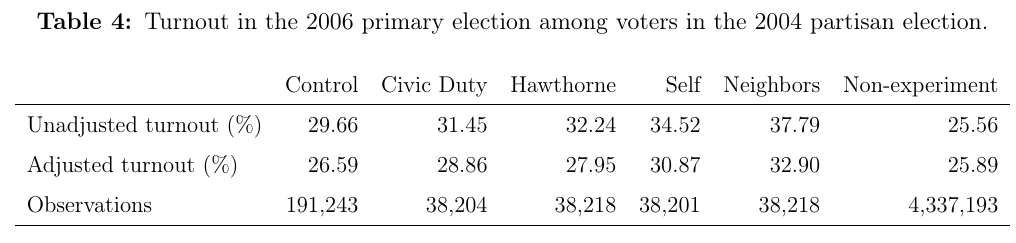
\includegraphics[width=0.99\textwidth]{figures/saevje-table4.png}
    % \caption{\label{fig:label} }
  \end{figure}


\end{frame}



% -------------------------------------------------------------------------

\begin{frame}
  \frametitle{Differences between Nattino et al. and S\"avje et al. }
  
  \begin{itemize}
  \item Nattio et al. \medskip 
    \begin{itemize}
    \item Attempt to mimic block randomization design \medskip 
    \item Adapts existing matched pair algorithm \medskip 
    \item Fisher randomization paradigm \medskip 
    \item Frequentist test and confidence intervals are standard \medskip 
    \end{itemize}
  \item S\"avje et al. \medskip 
    \begin{itemize}
    \item Less conventional experimental design $\rightarrow$ more
      researcher degrees of freedom (how to set $c_x$?) \medskip 
    \item Novel algorithm which generalizes full matching \medskip 
    \item Direct comparison of average outcomes \medskip 
    \item Quantifying uncertainty appears difficult, and is not
      attempted by the authors
    \end{itemize}
  \end{itemize}
  
\end{frame}


%%% Local Variables
%%% Local Variables:
%%% mode: latex
%%% TeX-master: "../main"
%%% End:
